\section{Timeline}
\label{sect:timeline}

Figure~\ref{fig:timeline} shows the timeline for 2D DRP tasks over the development, commissioning and operations phases of the PFS project, assuming
contributions could be made from a group of workers at NOAJ and IPMU, along with workers at Princeton.

There are 5 vertical lines. From the left, the grey vertical line indicates the date at which the first complete Spectrograph Module, including the Blue, Red and Near-Infrared detectors will be available at LAM. The vertical green lines indicate the start and end of engineering observations. The vertical black line indicates the call for SSP proposals.

The remaining lines in the top two-thirds of the diagram show timelines for 2D DRP tasks. 
The red and yellow horizontal lines in the bottom part of the diagram
show the timelines for key project and hardware activities. 

\begin{sidewaysfigure}[ht]
    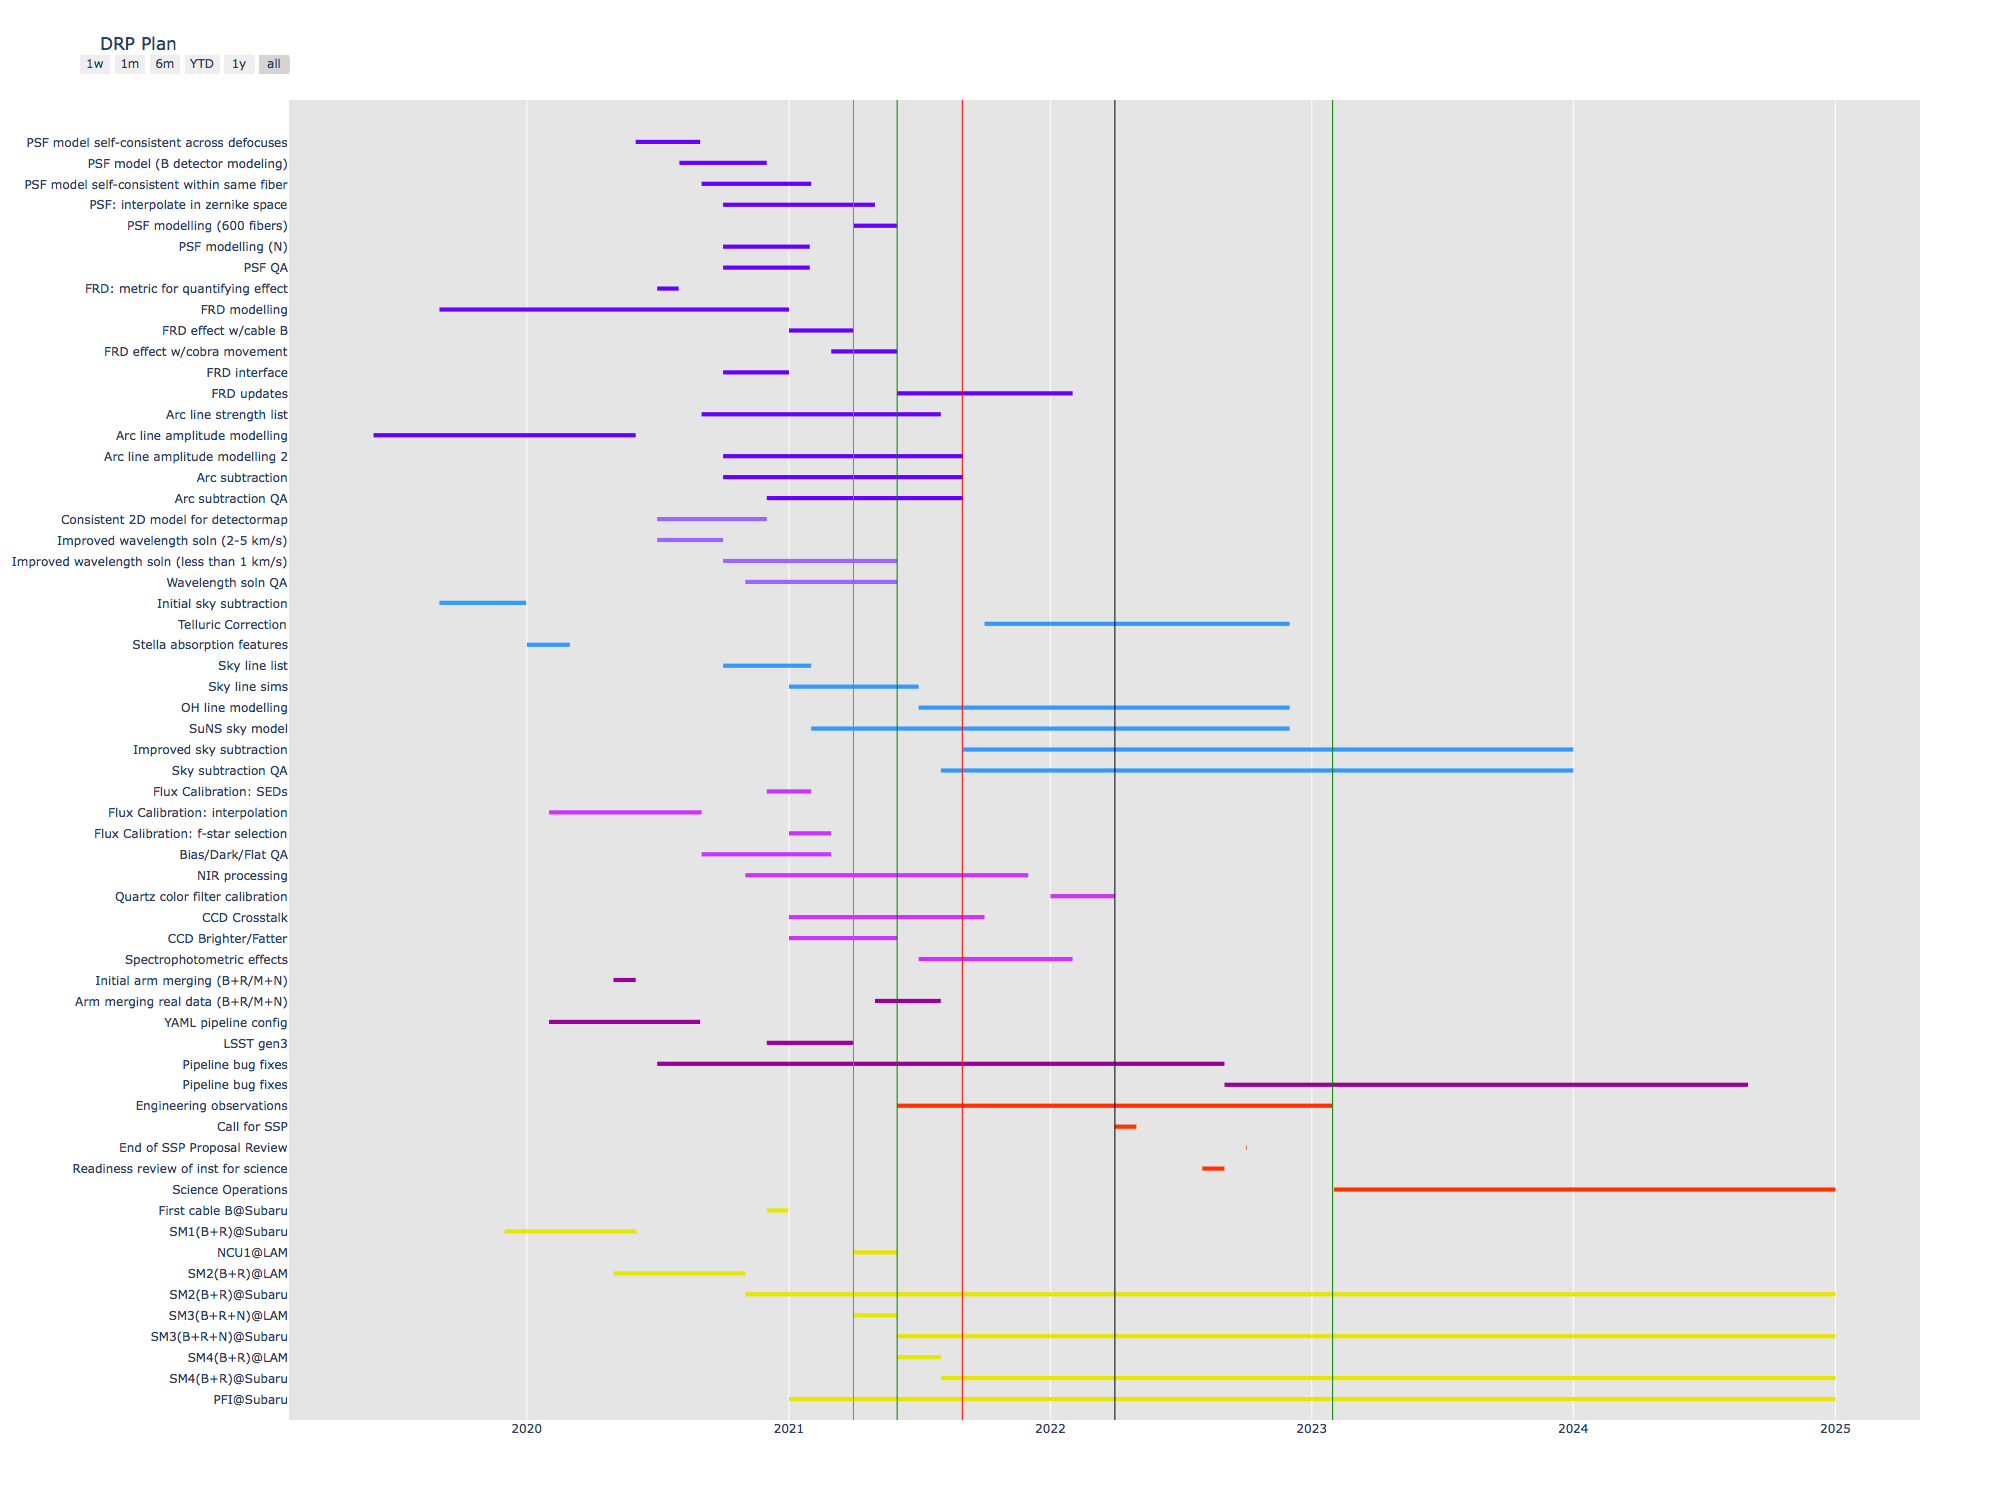
\includegraphics[width=25cm, height=20cm]{drp-timeline}
    \caption{2D DRP timeline. See text for description}
    \label{fig:timeline}
\end{sidewaysfigure}
\clearpage

\clearpage

